% Academic captions for the v5 figures.  Compile with the paper; paths are
% relative to the paper root (adjust if the figures live elsewhere).

\begin{figure}[t]
  \centering
  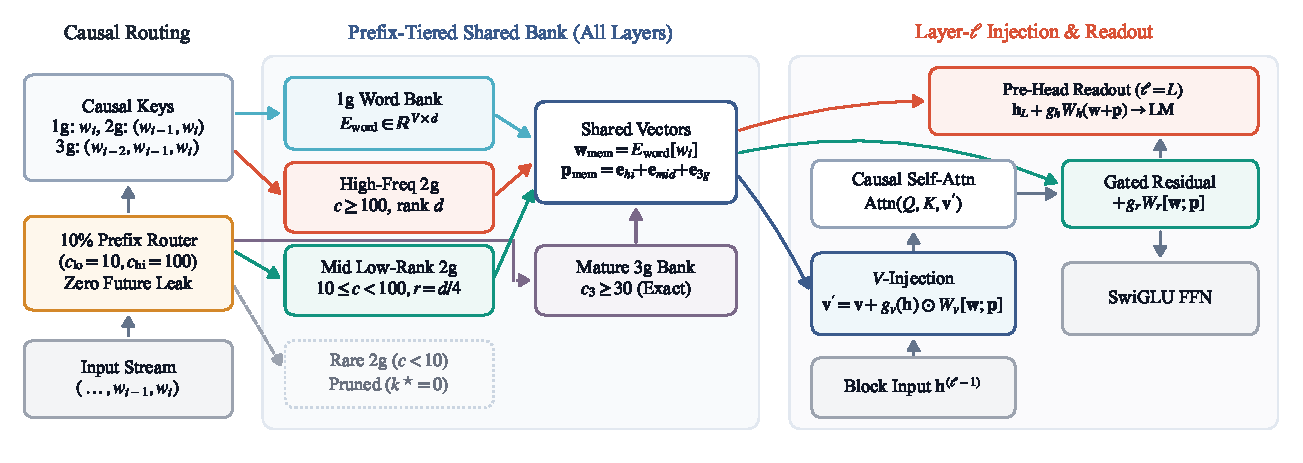
\includegraphics[width=\linewidth]{figs_v5/fig0_architecture.pdf}
  \caption{Shared prefix-tiered conditional value memory (\texttt{U123}).
  A 10\% prefix router allocates causal keys to a shared multi-granularity bank
  (1-gram, full-rank exact high-frequency 2-gram, low-rank mid-frequency 2-gram,
  and exact 3-gram) injected into attention values, residual streams, and a
  final pre-head readout.}
  \label{fig:arch}
\end{figure}

\begin{figure}[t]
  \centering
  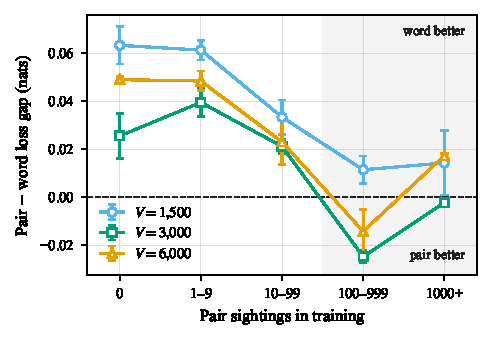
\includegraphics[width=\linewidth]{figs_v5/fig1_crossover.pdf}
  \caption{Word- versus pair-keyed value memory across pair-sighting buckets.
  Points show the mean gap (pair loss minus word loss; positive means the word
  table is better) at 300 training steps for three vocabularies; error bars are
  s.e.m.\ over three seeds.  Word tables lead on pairs seen fewer than 100
  times, and pair tables lead in the 100--999 bucket.  The 1000+ bucket is
  mixed in these runs (see Section~X); we therefore state the crossover as a
  range, not as a sharp universal threshold.}
  \label{fig:crossover}
\end{figure}

\begin{figure}[t]
  \centering
  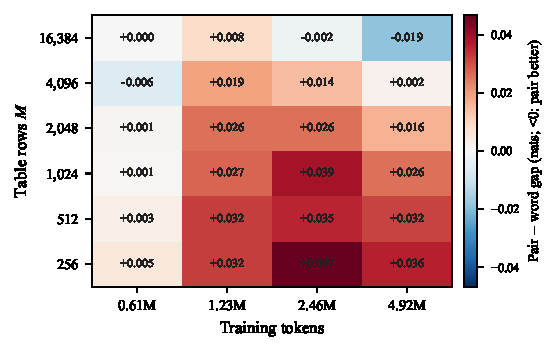
\includegraphics[width=\linewidth]{figs_v5/fig2_phase.pdf}
  \caption{Collision--variance phase diagram at $V=1{,}500$.  Cell colour is the
  pair-minus-word loss gap (negative, blue: pair tables better); numbers are the
  same gap in nats.  Pair tables cross over only when both the number of table
  rows $M$ and the number of training tokens are large; with $M\le2{,}048$ the
  collision bias prevents a crossover in this grid.}
  \label{fig:phase}
\end{figure}

\begin{figure}[t]
  \centering
  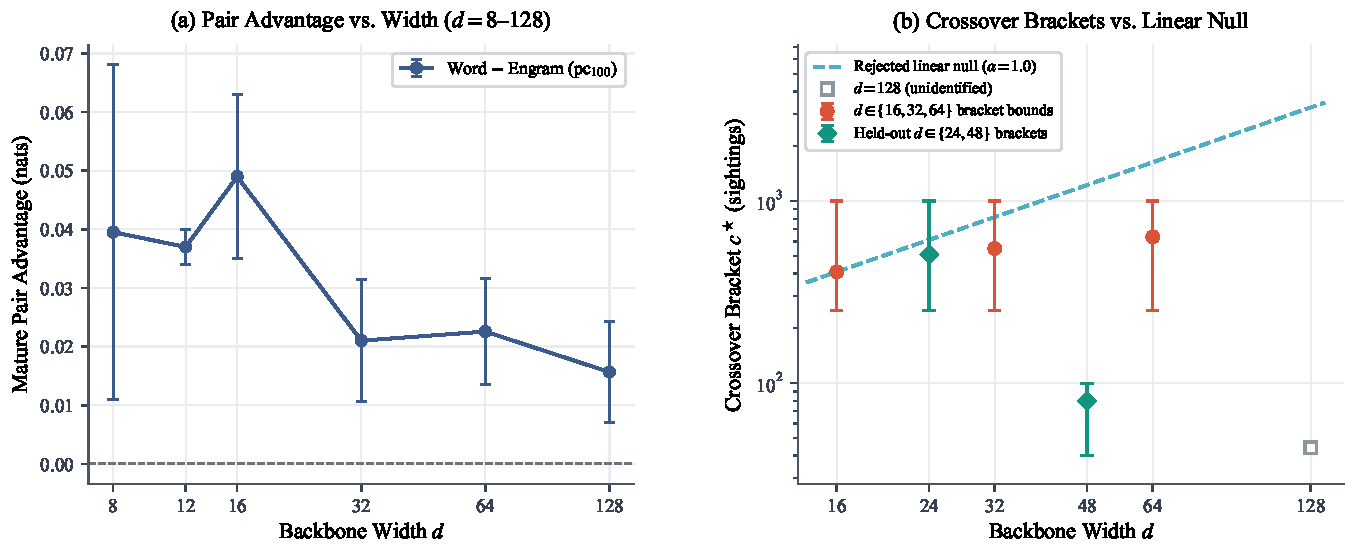
\includegraphics[width=\linewidth]{figs_v5/fig3_width_cstar.pdf}
  \caption{(a) High-frequency pair advantage (word minus Engram loss in the
  100--999 bucket) versus model width.  The advantage narrows as the model
  widens.  (b) Interval-bracketed crossover thresholds $c^\star(d)$ versus
  width alongside the linear null ($\alpha=1.0$).  Across $d\in\{16,24,32,64\}$
  crossings stay within $[250, 1000]$ and $d=128$ is unidentified; bootstrap
  power-law CIs span zero ($[-1.20, +0.96]$, $R^2=0.455$ with $d=128$), so we
  report bracket bounds and reject linear scaling ($P(\alpha\ge 1)=0.0247$;
  held-out $d=24,48$ stay positive on \texttt{b\_500\_1000}) without claiming a
  point-estimate power law.}
  \label{fig:width}
\end{figure}

\begin{figure}[t]
  \centering
  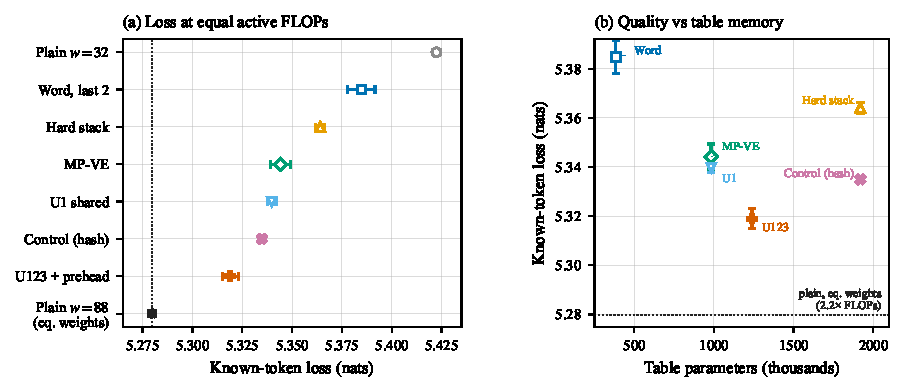
\includegraphics[width=\linewidth]{figs_v5/fig4_method.pdf}
  \caption{(a) Known-token loss at $L=4$, $w=32$, $V=6{,}000$ (300 steps,
  three seeds; error bars are s.e.m.).  The dotted line marks the plain model
  widened to the same total parameter count.  (b) Loss versus table parameters.
  U1 (shared memory across four layers) is the latency-efficient variant; U123
  (maturity routing plus pre-head readout) has the best loss among table methods
  but is slower.  The equal-weight plain model still has the best loss at
  $2.2\times$ the active FLOPs, so the method is positioned for
  equal-active-FLOPs, compute-limited inference rather than equal weights.}
  \label{fig:method}
\end{figure}

\begin{figure}[t]
  \centering
  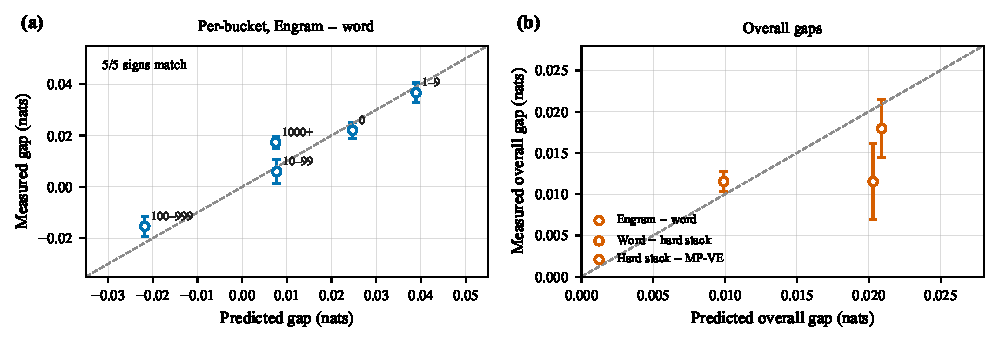
\includegraphics[width=\linewidth]{figs_v5/fig5_heldout.pdf}
  \caption{Preregistered held-out prediction at an unseen configuration
  ($V=4{,}500$, $d=48$, $L=4$, 250 steps $\times$ 128).  (a) Predicted versus
  measured per-bucket gaps (Engram minus word); all five bucket signs match.
  (b) Predicted versus measured overall gaps for three comparisons; the
  absolute errors are 0.0016, 0.0029 and 0.0088 nats, all below the
  preregistered 0.015-nat break threshold.}
  \label{fig:heldout}
\end{figure}

\begin{figure}[t]
  \centering
  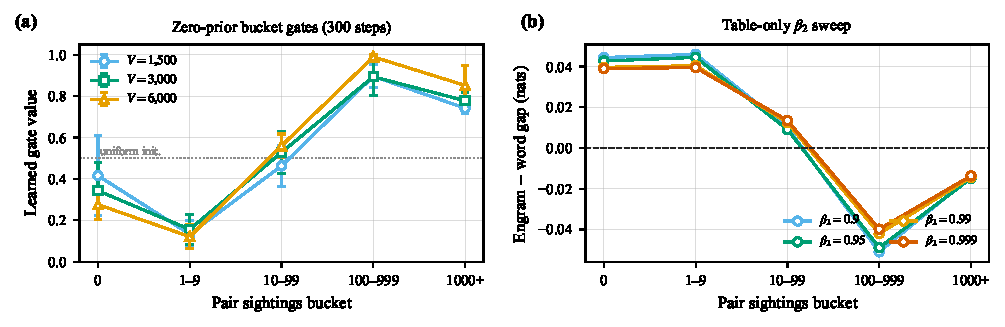
\includegraphics[width=\linewidth]{figs_v5/fig6_gates_beta2.pdf}
  \caption{(a) Bucket gates learned from a uniform initialisation of $0.5$ at
  300 steps (mean $\pm$ s.d.\ across seeds and layers).  The 0 bucket receives
  no training signal and remains near its initial value; the 1--9 bucket is
  suppressed and the 100+ buckets saturate.  (b) Table-only $\beta_2$ sweep.
  The crossover location is stable across $\beta_2\in[0.9,0.999]$; the
  magnitude attenuates by roughly 20\%.}
  \label{fig:gates}
\end{figure}

\begin{figure}[t]
  \centering
  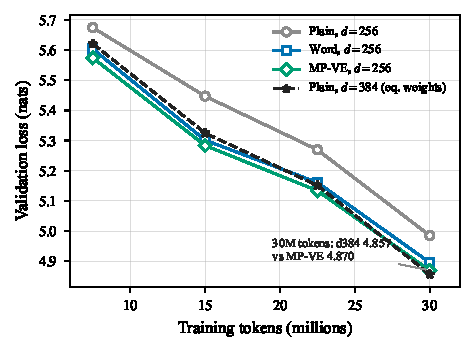
\includegraphics[width=\linewidth]{figs_v5/fig7_bridge.pdf}
  \caption{Full-vocabulary ($V=50{,}257$) bridge at $L=6$, $d=256$, 30M
  tokens (three seeds on \texttt{U123\_v2\_fullmid}, \texttt{CTRL\_hs\_pruned},
  \texttt{U123} low-rank, and \texttt{plain\_d384}; error bars show s.d.).
  (a) Replacing the low-rank mid bottleneck with full-rank hashed rows
  (\texttt{U123\_v2\_fullmid}, $4.8072\pm0.0099$) recovers $+0.0284$ ($t=2.54$)
  over original low-rank \texttt{U123} ($4.8355$) and beats $2.25\times$ compute
  \texttt{plain\_d384} by $+0.0527$ ($t=8.27$), but is statistically
  indistinguishable from co-main baseline \texttt{CTRL\_hs\_pruned}
  ($+0.0118\pm0.0163, t=1.25$). (b) Batch-16 inference throughput vs.\ loss frontier.}
  \label{fig:bridge}
\end{figure}

\begin{figure}[t]
  \centering
  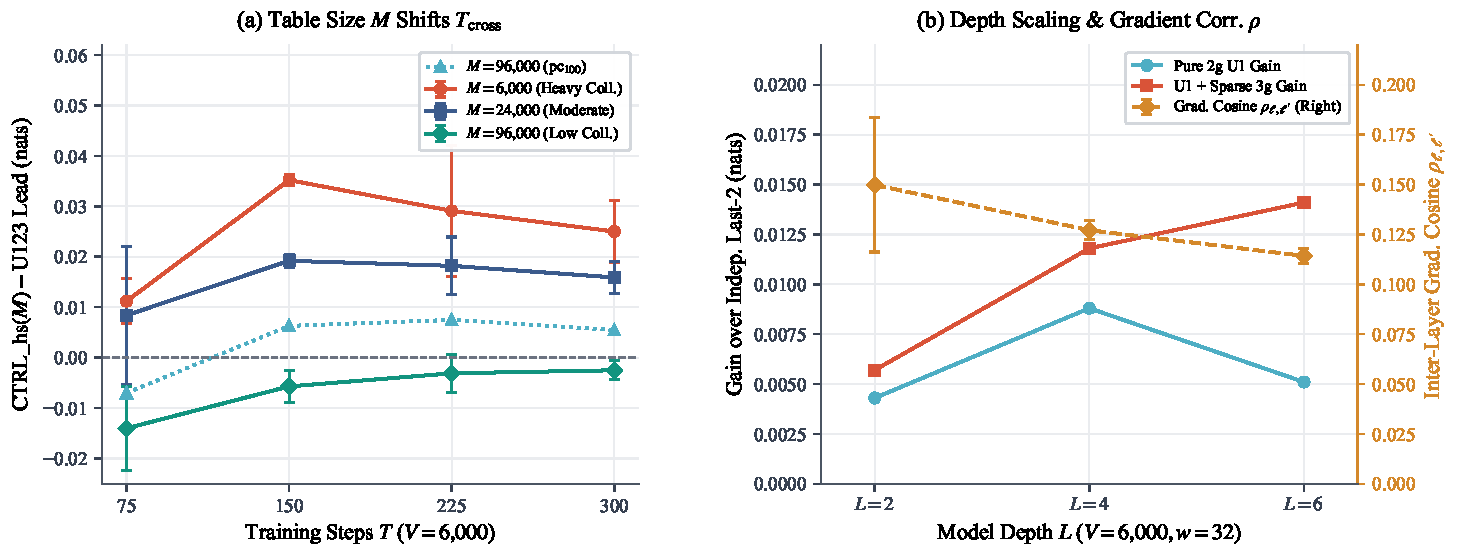
\includegraphics[width=\linewidth]{figs_v5/fig8_theory_tests.pdf}
  \caption{Phenomenological model tests ($L=4$, $w=32$, $V=6{,}000$, three seeds).
  (a) Relaxing hash table size $M$ from $6\text{k}$ to $96\text{k}$ shrinks
  \texttt{U123}'s global lead and shifts $T_{\mathrm{cross}}$ right while the
  mature \texttt{pc\_100} bucket still crosses cleanly. (b) Depth scaling ($L=2,4,6$)
  paired with 3-seed inter-layer gradient cosine $\rho_{\ell,\ell'}$ ($0.15\to 0.11$).}
  \label{fig:theory}
\end{figure}
